\section{Using it}
\label{sec:usage}

This section shows the tool from the outside: its commands, the one setting that matters most, and what a run returns. How the checks work inside is the subject of Section~\ref{sec:system}.

A check that nobody runs protects nobody. So LLossless sits where merges already happen: as a command in a script or a pipeline, and as a web page. It has two jobs. \texttt{llossless merge} asks a model to merge up to \ccnum{tool.max_sources} documents and then checks the result. \texttt{llossless verify} checks a merge that already exists, however it was made, and makes no merge call.

\begin{quote}\small\ttfamily
llossless merge a.md b.md -{}-base a.md -o merged.md > report.md\\
llossless verify a.md b.md merged.md > report.md
\end{quote}

\noindent In the first command \texttt{a.md} and \texttt{b.md} are the sources. \texttt{-{}-base} names the \emph{base}: the source whose structure the merged document follows. \texttt{-o} names the file the merged document is written to, and the report goes to standard output. The second command takes the sources and then the merge to be checked.

\paragraph{The web interface.} \texttt{llossless serve} runs the same merge and the same checks behind a small self-hosted server (Figure~\ref{fig:webui}). It has accounts that can each hold their own API keys, a model picker that shows measured cost, speed and silent loss per model with the date of the measurement and marks a model that the benchmark disqualified, and pages in English and German.

\paragraph{Three roles, and three ways to reach a model.} A model does up to three jobs in a run, and I call them roles. In the \emph{merge} role it writes the merged document. In the \emph{decompose} role it splits each document into \emph{claims}, which are short statements of one fact each. In the \emph{verify} role it compares each claim with the other side: a claim from a source with the merged document, and a claim from the merged document with the sources. Decompose and verify together are the judge. The roles can use different models, so an expensive model can write the merge while a cheaper one checks it.

A model can be reached through a local server that speaks the OpenAI API, through a vendor's API, or through a command-line program that runs under a subscription, such as Anthropic's Claude Code. A vendor's API is billed by the token, and a subscription is a fixed fee that buys a budget of usage (Section~\ref{sec:findings} comes back to the difference). The tool starts Claude Code in its safe mode, an option that loads none of the user's own configuration (Section~\ref{sec:lessons} says why).

\paragraph{How freely the merge may reword.} A merge that may only copy sentences is wrong when it rewrites one, and a merge that may edit freely is not. So one setting, the \emph{fidelity level}, tells the merge how much it may edit and tells the checks the same thing. There are \ccnum{tool.levels} levels, each allowing what the rows above it allow and more. The default is \texttt{\ccnum{tool.default_level}}, because I expect a model to improve how the merged text reads and flows. \texttt{verbatim} and \texttt{low} keep the text with little or no change, and I doubt that \texttt{verbatim} has much use in practice.

\begin{center}\small
\begin{tabular}{@{}lp{0.72\linewidth}@{}}
\toprule
Level & The merge may \\
\midrule
\texttt{verbatim} & only copy sentences, choosing which version to keep and in what order \\
\texttt{low} & also make mechanical corrections: spelling, punctuation, grammar \\
\texttt{mid} & also rewrite single sentences \\
\texttt{high} & also edit like a careful editor, state what the sources together entail, and choose one value where the sources disagree, with a record of the choice \\
\texttt{open} & also carry a value that covers both sources where they disagree, and state something from outside the documents, in a declared record that names what it rests on \\
\texttt{sourced} & as \texttt{open}, with the model looking facts up on the web instead of recalling them \\
\bottomrule
\end{tabular}
\end{center}

\noindent At \texttt{high} the merge may join facts from several documents into one statement, and where the sources disagree it may choose one value and record the choice, as the runbook merge did. Up to \texttt{mid} it may not choose, so a user who wants every disagreement kept on the page runs at \texttt{mid} or below. At \texttt{open} the merge may also state something that is in none of the documents, for example to correct an error in a source, which it would otherwise carry over. The tool cannot check such a statement against the documents, so the merge must declare each one with what it rests on, and the report lists them for a person to review.

\begin{figure}[H]
\centering
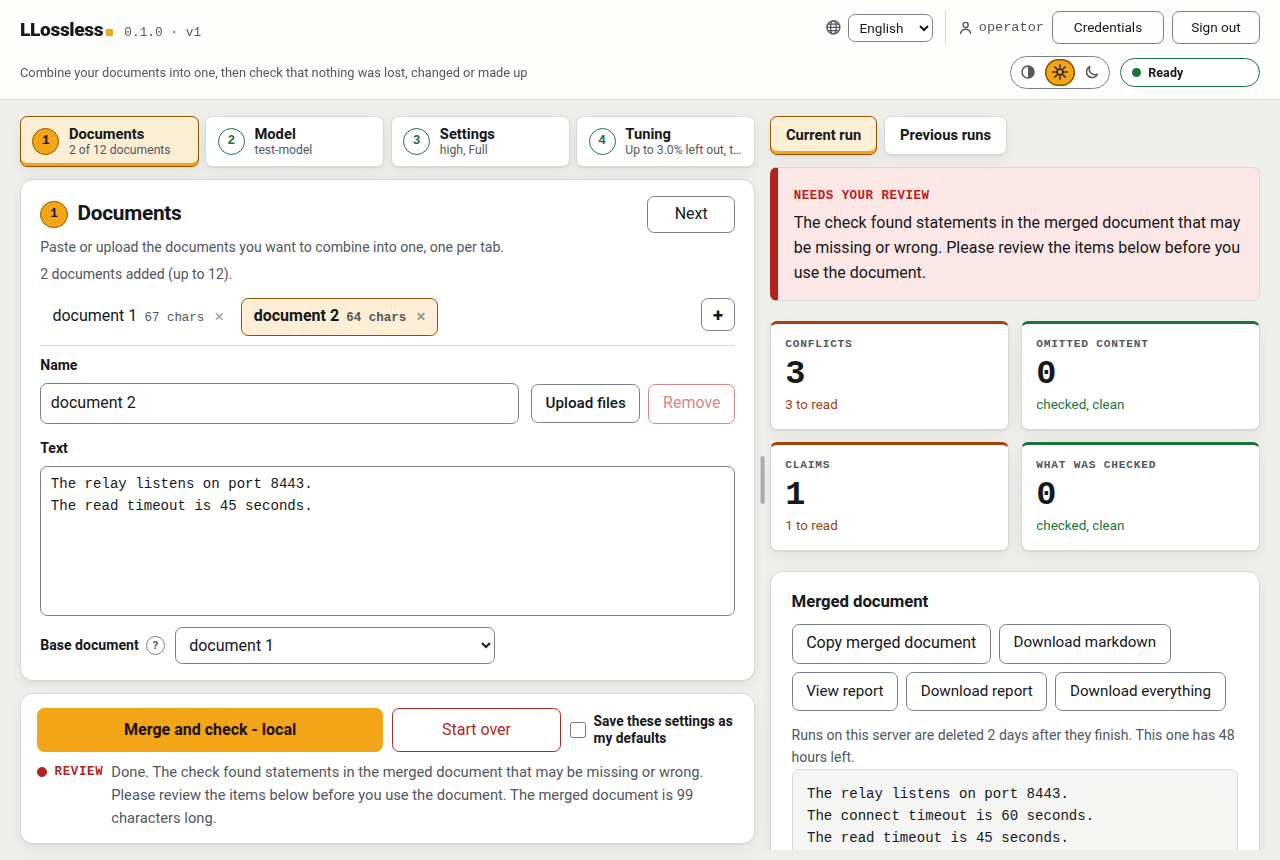
\includegraphics[width=\linewidth]{../docs/img/web-ui-light.png}
\caption{The web interface after a run with findings: the documents on the left, and on the right the findings, the checks that ran and the merged document with its downloads. The answers in this screenshot came from a scripted test endpoint, not from a real model.}
\label{fig:webui}
\floatfoot
\end{figure}

\paragraph{Rules that do not depend on the level.} In a merge the tool made, numbers, links, file paths, version strings and code must arrive character for character at every level. A changed one is a finding.

What a merge states from outside the documents has three possible outcomes at \texttt{open}, and the tool treats them differently:
\begin{points}
\item \emph{Declared, and the documents say nothing on the matter.} The statement is listed in the report for review. It is not a finding.
\item \emph{Declared, and it contradicts a source.} This is a correction. It is listed in the report, and it is still a finding that fails the run. The tool cannot tell a correction from an error, because the documents are the only reference it has.
\item \emph{Not declared.} The statement is reported as invented.
\end{points}

\noindent One run of the benchmark shows the second case. A source of the Voyager set says that the names of some newly found moons are ``obvious allusions to Goethe''. That is one of the errors I planted. At \texttt{open} the model wrote ``allusions to Shakespeare and Alexander Pope'' and declared the change. Shakespeare and Alexander Pope is the correct fact and Goethe is the error I planted, so the model put the planted error right. The report still lists the statement among those added from outside the documents. It also reports that the merge contradicts its source, and the run ends with exit code 1, because the tool cannot tell a correction from a contradiction. A person has to confirm the correction.

\paragraph{What comes back.} A run returns a report and an exit code. The report is in Markdown, and on request the same report comes as JSON or as a self-contained HTML page. It opens with a summary of what was found. Then come the findings. A \emph{finding} is an entry that names one problem. Each finding of the judged checks names the claim, its file and line, and the evidence quoted. Every claim that was drawn from the documents is listed with what became of it. A block at the end records which model answered in each role, the settings, the cost and whether document content left the machine.

The exit code tells a script how the run went:

\begin{center}\small
\begin{tabular}{@{}lp{0.80\linewidth}@{}}
\toprule
Code & Meaning \\
\midrule
0 & Nothing was found. \\
1 & There is a problem in the merged document. The runbook merge of the opening story ended this way. \\
2 & The run could not finish, or could not check everything. I call such a run \emph{inconclusive}. \\
3 & Milder than 1: the merged document passed every check, but the merge's records are wrong or incomplete. Example: a record says a sentence was replaced, and the sentence is still in the merge unchanged. Or the sources head the same section differently, and the merge kept one heading and wrote no record for the other. \\
\bottomrule
\end{tabular}
\end{center}

\noindent When more than one applies, the run returns the most serious: 2 before 1, and 1 before 3. An inconclusive run is not a pass. A run that checked nine claims of twelve has not shown the merge clean, so any unfinished part makes the whole run inconclusive.
